\chapter{Laplace transform}
Up until this point, the project has focused on the behaviour of electrical circuits in the time domain. Observing how different signals change with time yielded a differential equation, as seen in section (\ref{sec371}).
\\ \\
The solution to a differential equation will often be difficult to derive, and this is where the Laplace transform comes in handy. The Laplace transform converts functions of time to functions of frequency (i.e. from the time domain to the \textit{s}-domain). This process reduces the differential equation in question to an algebraic equation. Once the expression has been solved in the \textit{s}-domain, the inverse Laplace transform can be applied to find its corresponding solution in the time domain. Generally, this description can be illustrated in the following way:
\begin{figure}[H]
\center
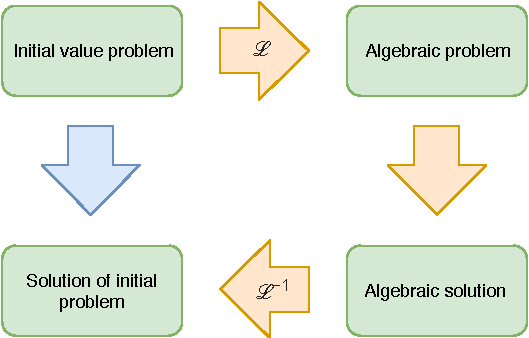
\includegraphics[scale=1]{fig/img/laplace_circ.pdf}
\caption{Solution using Laplace}
\label{lpsol}
\end{figure}

\section{The Laplace Transform}
\begin{definition}{Laplace transform}{}
\begin{align}
\mathcal{L}\{f(t)\}=F(s)=\int_{0}^{\infty} e^{-st}\cdot f(t)\ dt
\label{lpdef}
\end{align}
where $f(t)$ is a function of time, $F(s)$ is the Laplace transform of that very function, and $s$ is a complex variable.
\end{definition}
Since the definition consists of an improper integral (integral consisting of infinity), it can be rewritten as:
\begin{align}
\int_{0}^{\infty} e^{-st}\cdot f(t)\ dt = \lim_{N \to \infty} \int_{0}^{N} e^{-st}\cdot f(t)\ dt
\end{align}
When solving something like this, it has to be taken into consideration when the integral converges and diverges. Generally, a function converges when it approaches a specific value. A function diverges when it does not approach a specific value, e.g. when approaching infinity.

\begin{theorem}{Existence of the Laplace transform}{}
The function $f$ is said to be of exponential order if there exist nonnegative constants $M$, $c$, and $T$  such that $$|f(t)| \leq Me^{ct} for t \geq T.$$
Thus a function is of exponential order provided that it grows no more rapidly than a constant multiple of some exponential with a linear exponent. \cite[p. 320]{diffandcomplex}
\end{theorem}
\begin{prof}{}{}
Since $f$ is of exponential order, then $|f(t)| \leq Me^{ct}$ for all $t \leq 0$. Note that  $s=a+ib$. It follows that $$\lim_{N \to \infty} \int_{0}^{N} |f(t)|\cdot e^{-st}$$
\end{prof}
\begin{example}{Laplace transform for $e^{at}$}{lpe}
In (\ref{lpdef}), let $f(t)=e^{at}$, where $a$ is a constant, and $t$ is time. In that case,
$$\mathcal{L}\{f(t)\}=\int_{0}^{\infty} e^{-st}\cdot e^{at}\ dt$$
Since they have the base, $e$, in common, their exponents can be combined. Additionally, $t$ can be factorised:
$$\mathcal{L}\{f(t)\}=\int_{0}^{\infty} e^{-(s-a)t}\ dt$$
Since it is an improper integral, the limits are applied. This means that some number is set to approach infinity. Here N is set to approach $\infty$:
$$\mathcal{L}\{f(t)\}=\lim_{N \to \infty} \int_{0}^{N} e^{-(s-a)t}\ dt$$
Integration by substitution is now applied. Let $\dfrac{du}{dt}=-(s-a)$. This yields $dt=-\dfrac{1}{s-a}du$. The integral is now no longer from 0 to $\infty$, since new limits are applied. It is now an integral from $u=-(s-a)0=0$ to $u=-(s-a)N$. Since $-\dfrac{1}{s-a}$ is a constant it can be moved outside the integral. It is going to look like this:
\begin{align}
\mathcal{L}\{f(t)\}=\lim_{N \to \infty} \int_{0}^{-(s-a)N} e^{u}\cdot -\dfrac{1}{s-a}\ du = \lim_{N \to \infty} -\dfrac{1}{s-a} \cdot \left[e^{u} \right]_{0}^{-(s-a)N}
\label{eq6.2}
\end{align}
Now applying $u=0$ and $u=-(s-a)N$ to $e^{u}$:
\begin{align*}
\mathcal{L}\{f(t)\} =\lim_{N \to \infty} -\dfrac{1}{s-a}\cdot (e^{-(s-a)N}-e^{0})
\end{align*}
Since $e^{-(s-a)N}$ will approach $0$, when $N$ is approaching $\infty$ (if $Re(s) \geq a$). Therefore the equation is going to look as follows:
\begin{align}
\mathcal{L}\{f(t)\} = \dfrac{1}{s-a}
\end{align}
In conclusion, the Laplace transform of $f(t)=e^{at}$ equals
$$\mathcal{L}\{f(t)\}=\dfrac{1}{s-a} \ \ \ ;\ \ \ s>a$$
$s$ must be greater than $a$, since the limit of $e^{-(s-a)N}$ converges towards zero. If $a$ is greater than $s$, the exponent of $e$ would be positive, and the limit would diverge.
\end{example}
The Laplace transform can be used for all functions of $f$, where the real part of $s$ is greater than $a$ $Re(s) \geq a$. Since $s$ is a complex number ($s=a+ib$), only the first part of $s$ has to be greater than $a$. Therefore, $e^{-st}$ is  the same as $e^{-ta}e^{-tib}$, where the last part is the imaginary part of the complex number. In the complex chapter, this is also defined as $e^{a}\cos(b)+ i \sin(b)$. Since the imaginary parts are defined as functions of cosine and sinus, they can not approach $\infty$. Therefore, only the real part of $s$ from equation \eqref{lpdef} can approach $\infty$, and is only going to converge when $Re(s) \geq a$, and diverge when $Re(s)<a$.
\\ \\
When doing the inverse Laplace transformation, the results can often be found by looking at the results from on ordinary Laplace transformation.
\begin{example}{Inverse Laplace transform}{}
Let $F(s) = \dfrac{4}{s+10}$. When recognizing this takes the same form as the result above, the solution becomes clear. Now this has to be put on the form $f(t)=e^{at}$, where 10 in this case is the constant. The result is therefore: \cite[p. 323]{diffandcomplex}
\begin{align}
\mathcal{L}^{-1}\{F(s)\} = 4e^{-10t}
\end{align}
\end{example}
The Laplace transform can be applied to the derivatives of multiple orders. In particular, the Laplace transform of the first order derivative, since it is essential when looking at the high and low-pass filters.
%mere tekst/bedre overgang
\begin{theorem}{Laplace transform of a first order derivative}
The Laplace-transform of a first order derivative takes the following form:
$$\mathcal{L}\{\frac{df}{dt}\} = s\cdot F(s)-f(0)$$
\end{theorem}
The Laplace transform of the first derivitive is using the rule of integration by parts. The rule states the following:
\begin{align}
\int_{a}^{b}{u(t) \cdot v(t)}=\left[u(t) \cdot v(t) \right]_{a}^{b}-\int_{a}^{b} \frac{du}{dt}\cdot v dt\
\label{eq6.3}
\end{align}

\begin{prof}{Laplace transform of a first order derivative}{lpderiv}
From the definition of a Laplace transform in equation \ref{lpdef}, the $u$ and $v$ from \ref{eq6.3} are chosen as: $u=e^{-st}$ and $v=f(t)$.
From the equation \ref{eq6.3} the following values are set: $u=e^{-st}$ and $v=f(t)$.
In this case, $u=e^{-st}$ and $v=f(t)$. Furthermore, infinity is replaced with the limit of some value N approaching $\infty$. This yields:
$$\mathcal{L}\{\frac{df}{dt}\}=\lim_{N \to \infty} \left(\left[e^{-st}\cdot f(t)\right]_{0}^{N}-\int_{0}^{N} -s\cdot e^{-st}\cdot f(t)\ dt \right)$$
To rewrite this rule is being used: $\frac{1}{a^n}=a^{-n}$. Additionally, since $s$ is merely a constant, it can be placed in front of the integral, such that:
\begin{align}
\mathcal{L}\{\frac{df}{dt}\}=\lim_{N \to \infty} \left[\dfrac{1}{e^{st}}\cdot f(t)\right]_{0}^{N}+ \lim_{N \to \infty} \left(s\cdot \int_{0}^{\infty}e^{-st}\cdot f(t)\ dt \right)
\label{eq6.4}
\end{align}

Note, that the second term of (\ref{eq6.4}) now equals the product of $s$ and $\mathcal{L}\{f(t)\}$.
$$\mathcal{L}\{\frac{df}{dt}\} = \lim_{N \to \infty}\left[\dfrac{1}{e^{s\cdot N}}\cdot f(N)-\dfrac{1}{e^{s\cdot 0}}\cdot f(0)\right]+s\cdot \mathcal{L}\{f(t)\}$$
FORKLARING ME BLA BLA BLA PROOF REFERENCE
Since $$\lim_{N \to \infty}\left[\dfrac{1}{e^{s\cdot N}}\right]=0$$ then, naturally, any other number multiplied by 0 will also equal to 0.\\
In conclusion, this results to
\begin{align*}
\mathcal{L}\{\frac{df}{dt}\} = s\cdot \mathcal{L}\{f(t)\}-f(0)
\end{align*}
\end{prof}
When taking a look back at the figure \ref{lpsol}, an example will show the advantage of the Laplace transform. In the following example with an initial value problem, the result is found with the Laplace transformation. Furthermore, it is going to show the difficulties connected with finding a result without the Laplace transformation.
\begin{example}{Laplace example}{laplaceexample}
In this example the following differential equation will be solved using the Laplace transformation:
\begin{align}
\dfrac{df}{dt}=e^{5t}, 	
\end{align} \label{inieq}
with the starting condition $f(0)=-1$. Sometimes an equation like that can be difficult to solve, and the Laplace transformation can be used. The Laplace transformation is applied on both sides:
\begin{align*}
\mathcal{L} \{\dfrac{df}{dt} \}= \mathcal{L} \{e^{5t} \}
\end{align*}
The Laplace transform of the derivative is inserted from \ref{lpderiv}, and the Laplace transform of $e^{5t}$ is inserted from \ref{lpe}:
\begin{align*}
s \cdot F(s) - f(0) = \dfrac{1}{s-5}
\end{align*}
Now $f(0)=-1$ is inserted:
\begin{align*}
s \cdot F(s) + 1 = \dfrac{1}{s-5}
\end{align*}
This value is now subtracted on both sides and put on a common denominator:
\begin{align*}
s \cdot F(s) = \dfrac{1-(s-5)}{s-5}
\end{align*}
Both sides are now divided by $s$ and the nomirator on the right side is simplified:
\begin{align*}
F(s) = \dfrac{6-s}{s(s-5)}
\end{align*}
Now the next step is to find the inverse Laplace transform. This is done using partial decompositition: \cite[p. 537]{calc}
\begin{align}
F(s) = \dfrac{6-s}{s(s-5)} = A \dfrac{1}{s} + B \dfrac{1}{s-5}
\label{par_dec}
\end{align}
Both sides of the expression above is now multiplied with the denominator of the left side $(s(s-5))$:
\begin{align*}
6 - s = A(s-5) + Bs
\end{align*}
Now this is split up in elements that are multiplied by $s$ and elements that are not:
\begin{align*}
6 - s = s(A+B) - 5A
\end{align*}
Now two equations with two unknown variables are created:
\begin{align*}
-5A &= 6 \Leftrightarrow A = - \dfrac{6}{5}\\
A + B &= -1 \Leftrightarrow - \dfrac{6}{5} + B = -1 \Leftrightarrow B = \dfrac{1}{5}
\end{align*}
These values are now put on the equation \ref{par_dec}:
\begin{align*}
F(s) =  - \dfrac{6}{5} \cdot \dfrac{1}{s} + \dfrac{1}{5} \cdot \dfrac{1}{s-5}
\end{align*}
The inverse Laplace transform is now applied:
\begin{align*}
\mathcal{L} \{F(s)\} =  - \dfrac{6}{5} \cdot \mathcal{L} \{\dfrac{1}{s}\} + \dfrac{1}{5} \cdot \mathcal{L} \{\dfrac{1}{s-5}\}
\end{align*}
Now the solutions can be identified from the table INSERT TABLE!!!
\begin{align*}
f(t) = - \dfrac{6}{5} + \dfrac{1}{5}e^{5t}
\end{align*}
This result can be tested by taking the derivative of $f(t)$ and inserting it on \ref{inieq}:
\begin{align*}
\dfrac{df}{dt} \left(- \dfrac{6}{5} + \dfrac{1}{5}e^{5t} \right) &= e^{5t} \\
e^{5t} &= e^{5t}
\end{align*}
Hereby the solution to the equation \ref{inieq} is found using the Laplace transformation.
\end{example}
